\documentclass[11pt]{article}
\usepackage[margin=1in]{geometry}
\usepackage{enumitem}
\usepackage{hyperref}
\usepackage{graphicx}
\usepackage{array}
\usepackage{multicol}
\usepackage{longtable}
\usepackage{titlesec}
\usepackage{booktabs}
\usepackage{amsmath}
\usepackage{float}
\usepackage{sectsty}
\sectionfont{\fontsize{14}{16}\selectfont}
\subsectionfont{\fontsize{12}{14}\selectfont}


\begin{document}

\begin{center}
    \large \textbf{Sri Sivasubramaniya Nadar College of Engineering, Chennai} \\
    (An autonomous Institution affiliated to Anna University) \\
    \vspace{0.3cm}
\end{center}

\begin{table}[!h]
\renewcommand{\arraystretch}{1.5}
\resizebox{\textwidth}{!}{%
\begin{tabular}{|l|cll|}
\hline
Degree \& Branch     & \multicolumn{1}{c|}{B.E. Computer Science \& Engineering} & \multicolumn{1}{l|}{Semester}        & V                                        \\ \hline
Subject Code \& Name & \multicolumn{3}{c|}{ICS1512 - Machine Learning Algorithms Laboratory}                                                                              \\ \hline
Academic year       & \multicolumn{1}{c|}{2025-2026 (Odd)}                        & \multicolumn{1}{c|}{Batch: 2023-2028} & \multicolumn{1}{c|}{\textbf{Due date: 29/7/25}} \\ \hline
\end{tabular}%
}
\end{table}

\vspace{0.5cm}

\begin{center}
 \textbf{Experiment 2: Loan Amount Prediction using Linear Regression}
\end{center}

\noindent
\section{Aim:} 
Apply Linear Regression to predict the loan amount sanctioned to users using the dataset provided.
 Visualize and interpret the results to gain insights into the model performance.

\vspace{0.4cm}
\noindent
\section{Libraries used:}
\begin{itemize}
    \item {Pandas}
    \item {Numpy}
    \item {Matplotlib}
    \item {Scikit-learn}
    \item {Seaborn}
\end{itemize}

\noindent
\section{Objective:} 
To evaluate the performance of a Linear Regression model in predicting loan sanction amounts based on applicant and property features. Model evaluation is done using 5-fold cross-validation and standard metrics (MAE, MSE, RMSE, R²).

\vspace{0.2cm}
\noindent
\section{Mathematical Description:} \\
\[
\hat{y} = \beta_0 + \beta_1 x_1 + \beta_2 x_2 + \dots + \beta_n x_n
\]
Where:
\begin{itemize}
    \item $\hat{y}$ = predicted loan amount
    \item $\beta_0$ = intercept
    \item $\beta_i$ = coefficient of feature $x_i$
\end{itemize}

We evaluate using the following metrics:
\begin{align*}
\text{MAE} &= \frac{1}{n} \sum_{i=1}^{n} |y_i - \hat{y}_i| \\
\text{MSE} &= \frac{1}{n} \sum_{i=1}^{n} (y_i - \hat{y}_i)^2 \\
\text{RMSE} &= \sqrt{\text{MSE}} \\
R^2 &= 1 - \frac{\sum (y_i - \hat{y}_i)^2}{\sum (y_i - \bar{y})^2}
\end{align*}

The objective is to minimize the cost function:

\[
J(\beta_0, \beta_1) = \frac{1}{n} \sum_{i=1}^{n} (y_i - (\beta_0 + \beta_1 x_i))^2
\]

\section{Code with Plot}
\begin{verbatim}
# 1. LOAD THE DATASET
import numpy as np
import pandas as pd
import matplotlib.pyplot as plt
import seaborn as sns
from sklearn.preprocessing import StandardScaler
from sklearn.model_selection import KFold
from sklearn.linear_model import LinearRegression
from sklearn.metrics import mean_absolute_error, mean_squared_error, r2_score

data = pd.read_csv('/content/drive/MyDrive/ml-lab/train.csv')
df = pd.DataFrame(data)
print(data.head())
\end{verbatim}

\vspace{0.4cm}
\textbf{OUTPUT:}
\begin{figure}[h!]
\centering
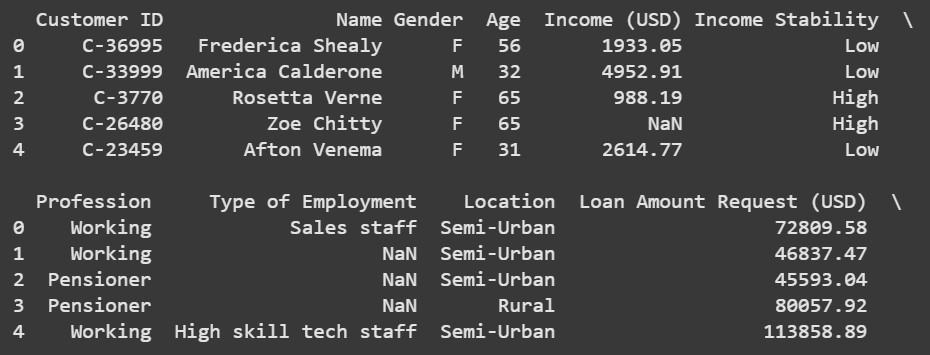
\includegraphics[width=0.9\textwidth]{expt2/dataset1.png} 
\end{figure}

\begin{figure}[h!]
\centering
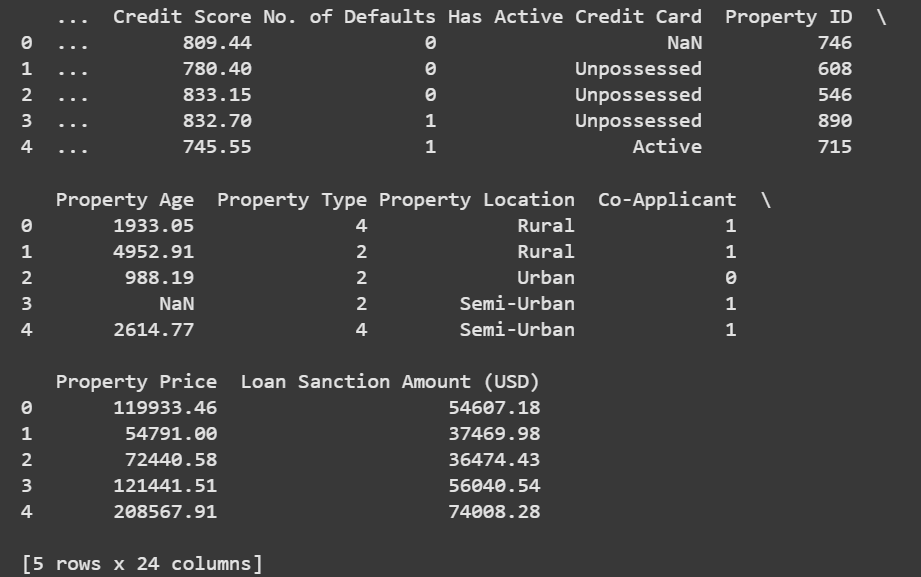
\includegraphics[width=0.9\textwidth]{expt2/dataset2.png} 
\caption{Dataset loaded}
\end{figure}

\begin{verbatim}
# 2. PREPROCESS THE DATA
# HANDLING MISSING VALUES
df['Credit Score'] = df['Credit Score'].fillna(df['Credit Score'].mean())
df['Current Loan Expenses (USD)'] = df['Current Loan Expenses (USD)'].fillna(df['Current Loan Expenses (USD)'].median())
df['Loan Sanction Amount (USD)'] = df['Loan Sanction Amount (USD)'].fillna(df['Loan Sanction Amount (USD)'].median())
df['Income Stability'] = df['Income Stability'].fillna(df['Income Stability'].mode()[0])
\end{verbatim}

\textbf{OUTPUT:}
\begin{figure}[h!]
\centering
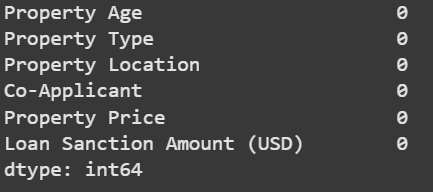
\includegraphics[width=0.9\textwidth]{expt2/missingvals.png} 
\caption{Missing values removed}
\end{figure}

\begin{verbatim}
# ENCODING CATEGORICAL VARIABLES
df = df.drop(['Customer ID', 'Name', 'Property ID'], axis=1)
df = pd.get_dummies(df, columns=['Gender', 'Profession', 'Location', 
'Property Location'], drop_first=True)

# ordinal variables = map
df['Income Stability'] = df['Income Stability'].map({'Low': 0, 'High': 1})
df['Expense Type 1'] = df['Expense Type 1'].map({'N': 0, 'Y': 1})
df['Has Active Credit Card'] = df['Has Active Credit Card'].map({
'Unpossessed': 0, 'Inactive': 1, 'Active': 2})

# high cardinality categorical variable = frequency encoding
emp_freq = df['Type of Employment'].value_counts(normalize=True)
df['Type of Employment Encoded'] = df['Type of Employment'].map(emp_freq)
df.drop('Type of Employment', axis=1, inplace=True)
\end{verbatim}

\textbf{OUTPUT:}
\begin{figure}[h!]
\centering
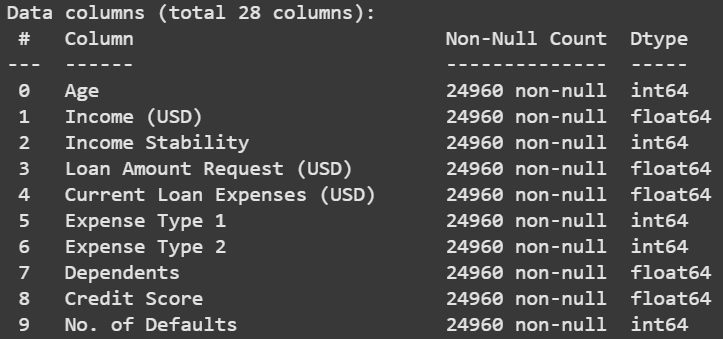
\includegraphics[width=0.9\textwidth]{expt2/encoded.png} 
\caption{Categorical variables encoded}
\end{figure}

\begin{verbatim}
# 3. EDA
sns.histplot(df['Loan Amount Request (USD)'], kde=True)
sns.boxplot(x='Gender_M', y='Loan Sanction Amount (USD)', data=df)

num_cols = df.select_dtypes(include=['float64']).columns
df[num_cols].hist(figsize=(15, 12), bins=30)
plt.tight_layout()

plt.figure(figsize=(15, 10))
sns.heatmap(df[num_cols].corr(), annot=True, fmt=".2f", cmap="coolwarm")
plt.title("Correlation Heatmap")
plt.show()
\end{verbatim}

\begin{figure}[H]
\centering
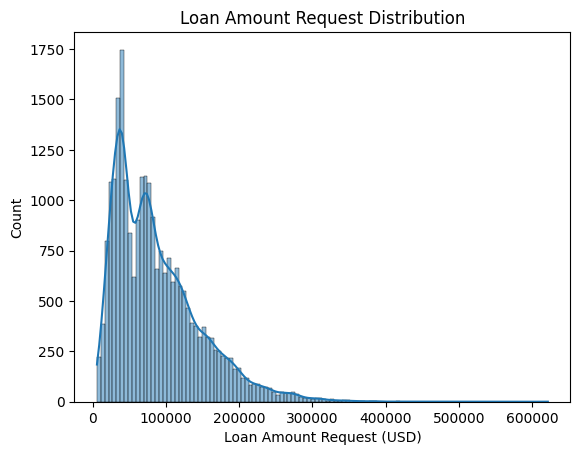
\includegraphics[width=0.8\textwidth]{expt2/loanhist.png} 
\caption{Loan Amount Request Distribution}
\end{figure}

\begin{figure}[H]
\centering
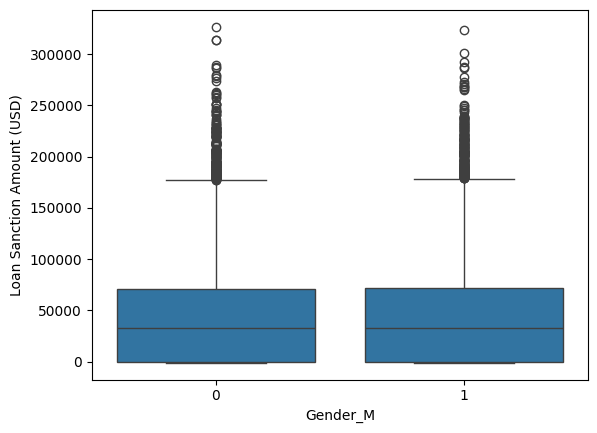
\includegraphics[width=0.8\textwidth]{expt2/genderbox.png} 
\caption{Gender boxplot}
\end{figure}

\begin{figure}[H]
\centering
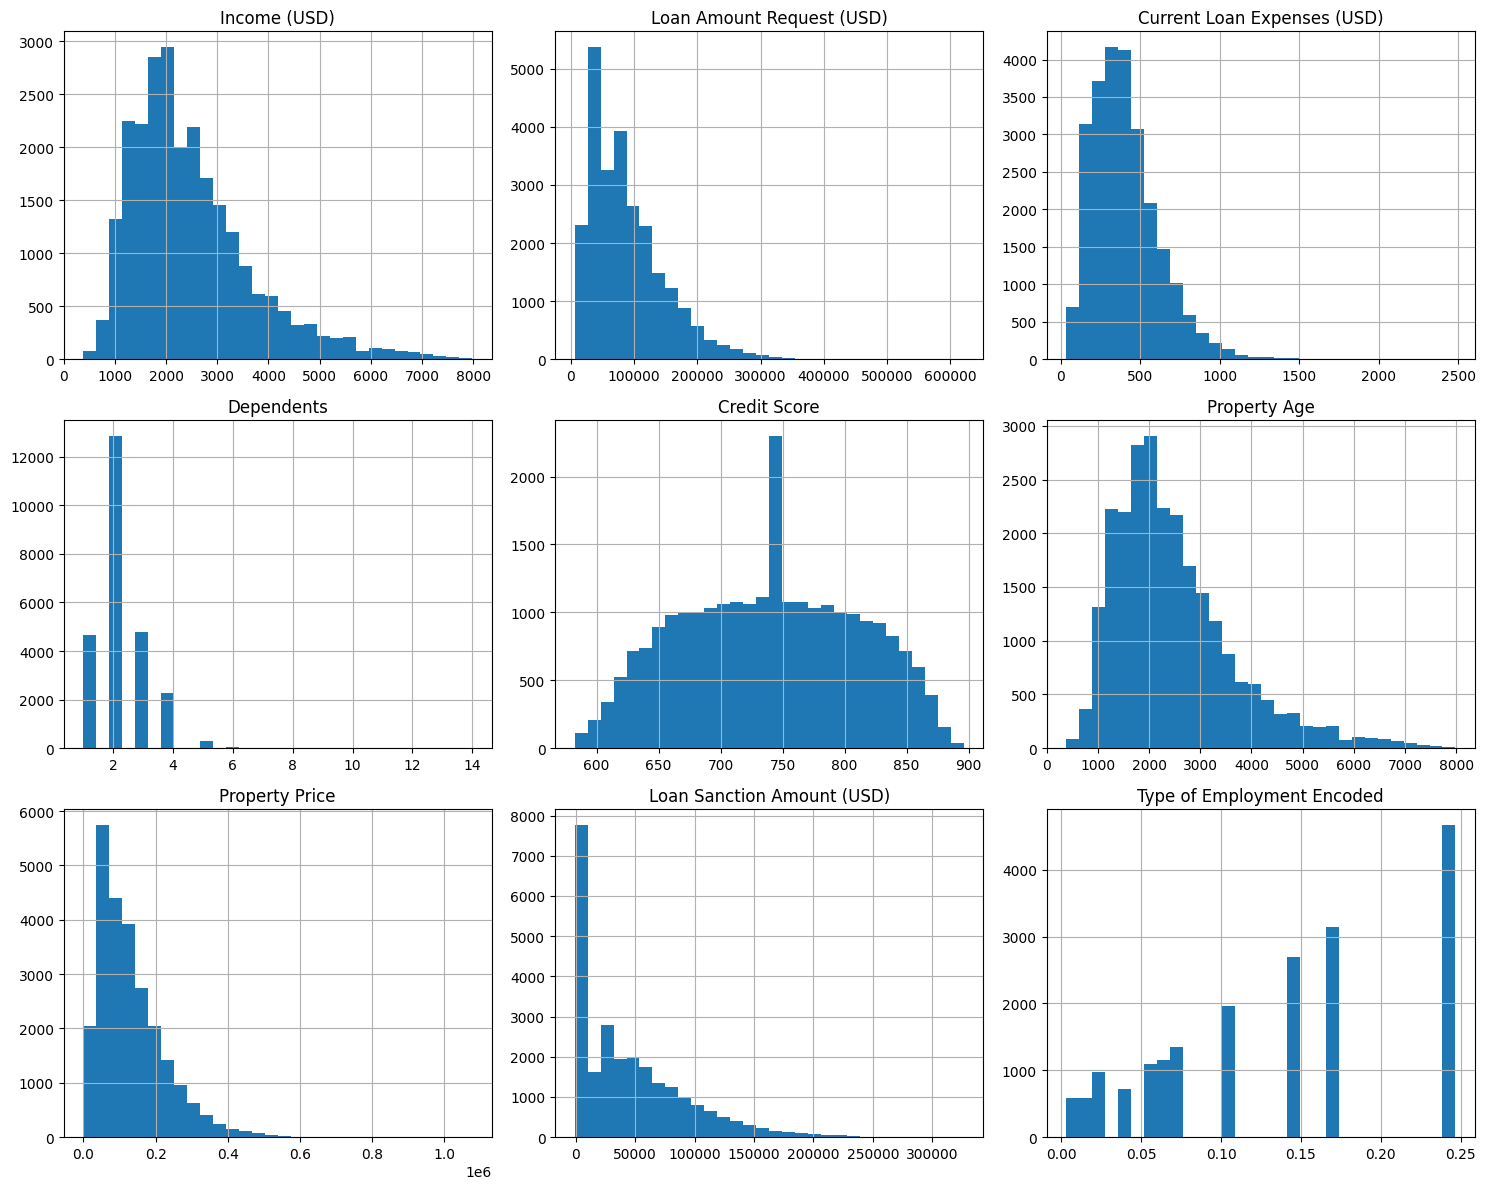
\includegraphics[width=0.7\textwidth]{expt2/hist.png} 
\caption{Histogram}
\end{figure}

\begin{figure}[H]
\centering
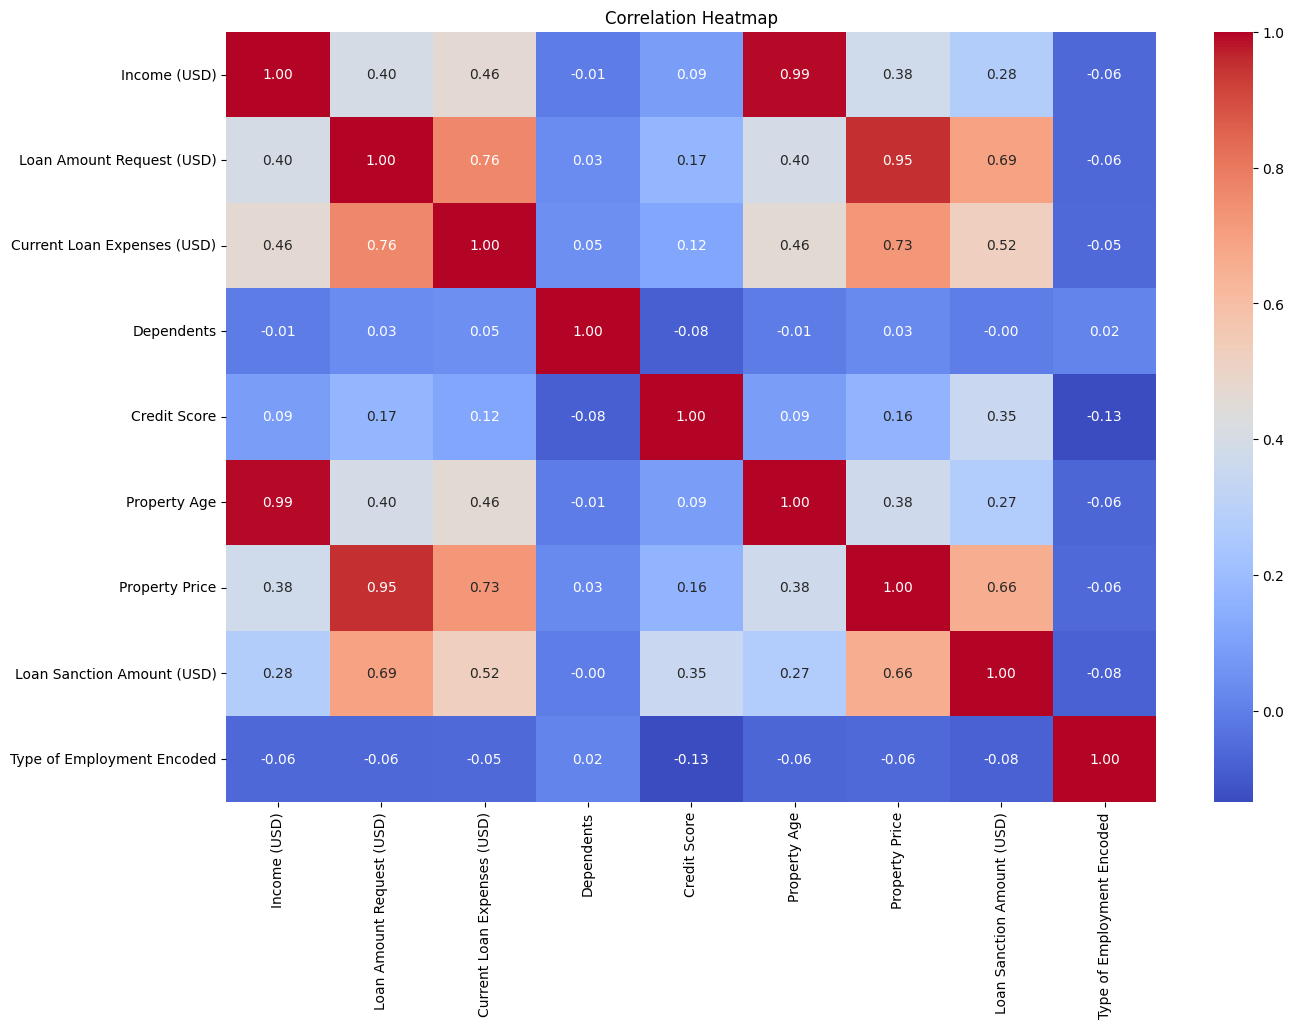
\includegraphics[width=0.8\textwidth]{expt2/heatmap.png} 
\caption{Correlation Heatmap}
\end{figure}

\begin{verbatim}
# 4. FEATURE ENGINEERING
scaler = StandardScaler()
num_cols = df.select_dtypes(include=['int64', 'float64']).columns  # picking only numerical cols, skip bool
df[num_cols] = scaler.fit_transform(df[num_cols])

# INTERACTION FEATURE
df['Affordability'] = np.log1p(df['Income (USD)'] / (df['Property Price'] + 1e-6))
df = df.dropna()

# 5. LINEAR REGRESSION - 5 FOLD CROSS VALIDATION
X = df.drop(columns=["Loan Sanction Amount (USD)"])  # everything except target
y = df["Loan Sanction Amount (USD)"]  # target variable

kf = KFold(n_splits=5, shuffle=True, random_state=42)
model = LinearRegression()

for fold, (train_index, val_index) in enumerate(kf.split(X), start=1):
    X_train, X_val = X.iloc[train_index], X.iloc[val_index]
    y_train, y_val = y.iloc[train_index], y.iloc[val_index]

    model.fit(X_train, y_train)
    y_pred = model.predict(X_val)

    mae = mean_absolute_error(y_val, y_pred)
    mse = mean_squared_error(y_val, y_pred)
    rmse = np.sqrt(mse)
    r2 = r2_score(y_val, y_pred)

    print(f"Fold {fold} - MAE: {mae:.2f}, MSE: {mse:.2f}, RMSE: {rmse:.2f}, R2: {r2:.4f}")

print("\nAverage MAE:", avg_mae)
print("Average MSE:", avg_mse)
print("Average RMSE:", avg_rmse)
print("Average R2:", avg_r2)
\end{verbatim}

\begin{figure}[H]
\centering
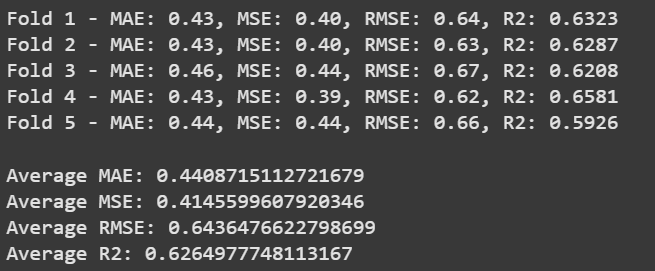
\includegraphics[width=0.7\textwidth]{expt2/metrics.png} 
\caption{Evaluation metrics}
\end{figure}

\begin{verbatim}
# 5. VISUALIZING RESULTS
plt.scatter(all_actuals, all_predictions, alpha=0.6, edgecolor='k')
plt.plot([all_actuals.min(), all_actuals.max()],
         [all_actuals.min(), all_actuals.max()])
plt.xlabel("Actual Loan Sanction Amount (USD)")
plt.ylabel("Predicted Loan Sanction Amount (USD)")
plt.title("Cross-Validation: Actual vs Predicted")
plt.grid(True)
plt.show()
\end{verbatim}

\begin{figure}[H]
\centering
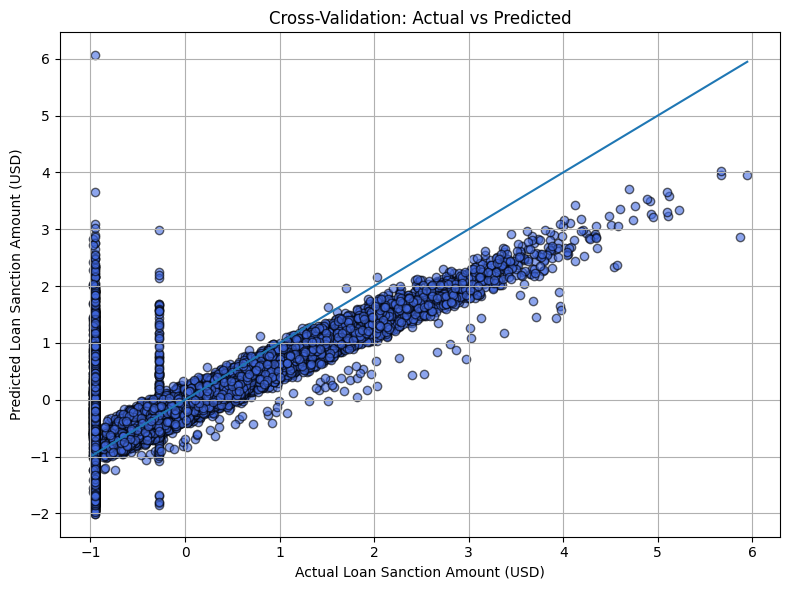
\includegraphics[width=0.7\textwidth]{expt2/actualpred.png} 
\caption{Actual vs Predicted}
\end{figure}

\begin{verbatim}
coeff_df = pd.DataFrame({
    'Feature': X_train.columns,
    'Coefficient': model.coef_
})

coeff_df = coeff_df.sort_values(by='Coefficient', key=abs, ascending=False)
sns.barplot(data=coeff_df, x='Coefficient', y='Feature')
plt.title("Feature Importance (Linear Coefficients)")
plt.grid(True)
plt.show()
\end{verbatim}

\begin{figure}[H]
\centering
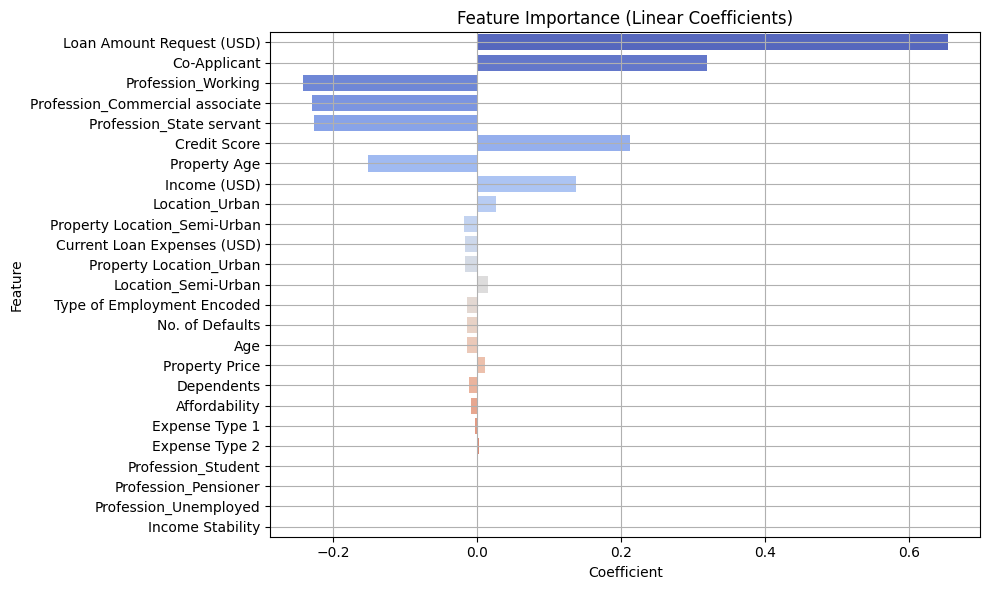
\includegraphics[width=0.8\textwidth]{expt2/featureimp.png} 
\caption{Feature Importance}
\end{figure}

\begin{verbatim}
residuals = all_actuals - all_predictions
plt.scatter(all_predictions, residuals, alpha=0.6)
plt.xlabel("Predicted Loan Sanction Amount (USD)")
plt.ylabel("Residuals")
plt.title("Cross-Validation: Residual Plot")
plt.grid(True)
plt.show()
\end{verbatim}

\begin{figure}[H]
\centering
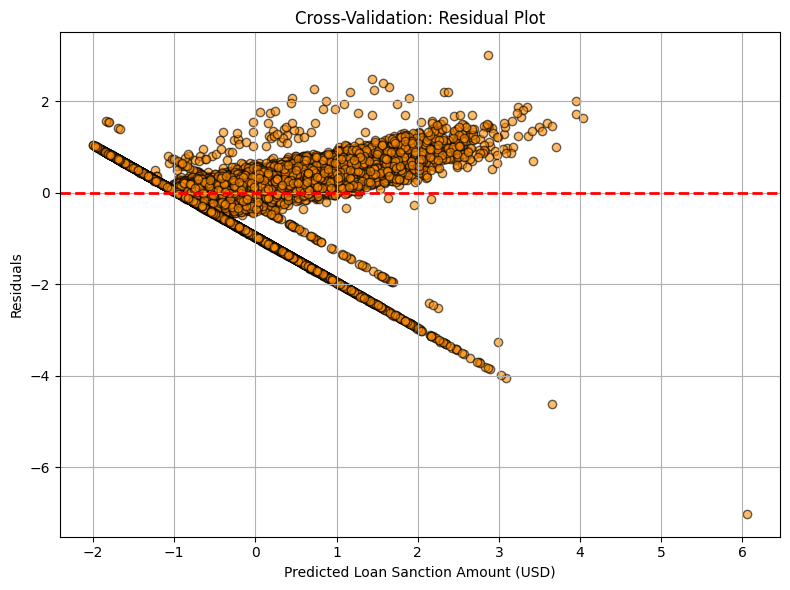
\includegraphics[width=0.7\textwidth]{expt2/residual.png} 
\caption{Residual Plot}
\end{figure}

\noindent
\section{Results Table:} \\
\begin{table}[H]
\centering
\begin{tabular}{|p{0.45\textwidth}|p{0.45\textwidth}|}
\hline
\textbf{Description} & \textbf{Student's Result} \\
\hline
Dataset Size (after preprocessing) &  24960 samples, 28 features

\\ 
\hline
Train/Test Split Ratio & 80:20 

\\ 
\hline
Feature(s) Used for Prediction &  All numeric and encoded categorical features

\\ 
\hline
Model Used & Linear Regression 

\\ 
\hline
Reference to CV Results Table & Table 1 

\\ 
\hline
Cross-Validation Used? (Yes/No) &  Yes

\\ 
\hline
If Yes, Number of Folds (K) &  5 

\\ 
\hline
Mean Absolute Error (MAE) on Test Set &  0.44087

\\ 
\hline
Mean Squared Error (MSE) on Test Set &  0.41455

\\ 
\hline
Root Mean Squared Error (RMSE) on Test Set &  0.64364\\ 
\hline
R2 Score on Test Set &  0.62649

\\ 
\hline
Most Influential Feature(s) & Loan Amount Request (USD), Credit Score, Co-Applicant, Income(USD) 

\\ 
\hline
Observations from Residual Plot &  Shows distinct non-random patterns and heteroscedasticity, indicating potential underfitting. Linear model may be too simple for the underlying data

\\ 
\hline
Interpretation of Predicted vs Actual Plot & While the model captures the general trend of loan sanction amounts, it struggles with accurate predictions for higher values 

\\ 
\hline
Any Overfitting or Underfitting Observed? &  Underfitting observed

\\ 
\hline
If Yes, Brief Justification (e.g., training vs test error, residual patterns) &  Consistent underprediction and limited variance in predicted values across actual ranges. Overly simplified predictions

\\ 
\hline
\end{tabular}
\caption{Summary of Results for Loan Amount Prediction}
\end{table}

\textbf{Cross-Validation Results Table:} \\
\begin{table}[h!]
\centering
\begin{tabular}{|l|c|c|c|c|}
\hline
\textbf{Fold} & \textbf{MAE} & \textbf{MSE} & \textbf{RMSE} & \textbf{R\textsuperscript{2} Score} \\
\hline
Fold 1 & 0.43 & 0.40 & 0.64 & 0.6323 \\
Fold 2 & 0.43 & 0.40 & 0.63 & 0.6287 \\
Fold 3 & 0.46 & 0.44 & 0.67 & 0.6208 \\
Fold 4 & 0.43 & 0.39 & 0.62 & 0.6581 \\
Fold 5 & 0.44 & 0.44 & 0.66 & 0.5926 \\
\hline
\textbf{Average} & 0.4409 & 0.4146 & 0.6436 & 0.6265 \\
\hline
\end{tabular}
\caption{Cross-Validation Results (K = 5)}
\end{table}

\section{Best Practices:} \\
\begin{itemize}
    \item \textbf{Used 5-Fold Cross-Validation} to ensure robust model evaluation and minimize bias from data splits.
    \item \textbf{Reported multiple evaluation metrics} (MAE, MSE, RMSE, and $R^2$) to provide a comprehensive assessment of model performance.
    \item \textbf{Observed consistent performance across folds}, indicating reasonable generalization and model stability.
    \item \textbf{No signs of overfitting}, as metrics remain relatively stable with no extreme deviations in any fold.
    \item \textbf{Rounded metric values} for readability in the table, while preserving precision in the backend calculations.
\end{itemize}

\section{Learning Outcomes}
\begin{itemize}
    \item Understood the implementation of 5-Fold Cross-Validation for evaluating model reliability.
    \item Gained experience interpreting regression metrics such as MAE, MSE, RMSE, and $R^2$.
    \item Identified the importance of consistency across folds to assess model stability.
    \item Learned to spot signs of overfitting or underfitting through performance trends.
    \item Developed a stronger grasp of model evaluation strategies used in real-world ML workflows.
\end{itemize}

\vspace{1cm}
\noindent
\textbf{GitHub Repository:} \\
\href{https://github.com/vidarshanaa15/ml-expt-2}{https://github.com/vidarshanaa15/ml-expt-2}

\end{document}